\section{Progettazione logica}
\subsection{Stima del volume dei dati}

\subsection{Descrizione delle operazioni principali e stima della frequenza}
Supponendo che ogni giorno ci siano 10 partite alla quale partecipano ogni volta 4 giocatori diversi. Le partite vengono sempre concluse in giornata e prevedono mediamente 70 tessere l'una.
\medskip

\centerline{\begin{tabular}{ |c|l|c| }
\hline
\textbf{Cod.} & \textbf{Operazione} & \textbf{Frequenza} \\
\hline
1 & Creare una nuova partita & 10 al giorno \\
\hline
2 & Visualizzare i server di gioco disponibili & 10 al giorno \\
\hline
3 & Visualizzare tutte le espansioni & 10 al giorno \\
\hline
4 & Creare un nuovo giocatore & 40 al giorno \\
\hline
5 & Visualizzare tutti i colori & 40 al giorno \\
\hline
6 & Ruotare la tessera corrente & 300 al giorno \\
\hline
7 & Piazzare la tessera corrente & 700 al giorno \\
\hline
8 & Piazzare o rimuovere un seguace su una sezione di una tessera & 350 al giorno \\
\hline
9 & Visualizzare i seguaci disponibili & 700 al giorno \\
\hline
10 & Assegnare dei punti ad un giocatore & 200 al giorno \\
\hline
11 & Aggiornare la tessera corrente & 700 al giorno \\
\hline
12 & Aggiornare il giocatore corrente & 700 al giorno \\
\hline
13 & Visualizzare le partire non concluse & 5 al giorno \\
\hline
14 & Visualizzare i giocatori di una partita & 70 al giorno \\
\hline
15 & Visualizzare le tessere piazzate & 5 al giorno \\
\hline
16 & Visualizzare le regioni in ordine di punteggio medio dei giocatori & 2 al mese \\
\hline
17 & Mostrare per ogni giocatore il numero di avversari con cui ha giocato & 4 all'anno \\
\hline
18 & Visualizzare per ogni regione l'espansione più giocata & 1 al mese \\
\hline
19 & Mostrare per ogni colore la probabilità statistica di vincere & 1 al giorno \\
\hline
\end{tabular}}

\subsection{Schemi di navigazione e tabelle degli accessi}

\subsection{Raffinamento dello schema}
(eliminazione di identificatori esterni, attributi composti e gerarchie, scelta delle chiavi)
\medskip

(elimanzione dell'attributo composto Position e l'inserimento delle due coordinate)

\subsection{Analisi delle ridondanze}

\subsection{Traduzione di entità e associazioni in relazioni}
\hspace{1.5em}players(\textbf{name})\newline

colors(\textbf{hex}, red, green, blue, name)\newline

games(\textbf{id}, server\_id, concluded)\newline
FK: server\_id REFERENCES servers(id)\newline

players\_in\_game(\textbf{player\_name}, \textbf{game\_id}, color\_hex, score, current, order)\newline
FK: player\_name REFERENCES players(name)\newline
FK: game\_id REFERENCES games(id)\newline
FK: color\_hex REFERENCES colors(hex)\newline

games\_expansions(\textbf{expansion\_name}, \textbf{game\_id})\newline
FK: game\_id REFERENCES games(id)\newline
FK: expansion\_name REFERENCES expansions(name)\newline

expansions(\textbf{name})\newline

meeple\_types(\textbf{name}, quantity, strength, expansion\_name)\newline
FK: expansion\_name REFERENCES expansions(name)\newline

meeples(\textbf{id}, owner\_player\_name, owner\_game\_id, type\_name, placed)\newline
FK: owner\_player\_name REFERENCES players\_in\_game(player\_name)\newline
FK: owner\_game\_id REFERENCES players\_in\_game(game\_id)\newline
FK: type\_name REFERENCES meeple\_types(name)\newline

gamesets(\textbf{id}, type\_name, points, closed)\newline
FK: type\_name REFERENCES gameset\_types(name)\newline

gameset\_types(\textbf{name}, starting\_points, endgame\_ratio, expansion\_name)\newline
FK: expansion\_name REFERENCES expansions(name)\newline

tile\_section\_types(\textbf{name}, next\_name*, previous\_name*)\newline
FK: next\_name REFERENCES tile\_section\_types(name)\newline
FK: previous\_name REFERENCES tile\_section\_types(name)\newline

tile\_sections(\textbf{type\_name}, \textbf{tile\_order}, \textbf{tile\_game\_id}, gameset\_id, meeple\_id*, closed)\newline
FK: type\_name REFERENCES tile\_section\_types(name)\newline
FK: tile\_order REFERENCES tiles(order)\newline
FK: tile\_game\_id REFERENCES tiles(game\_id)\newline
FK: meeple\_id REFERENCES meeples(id)\newline
FK: gameset\_id REFERENCES gamesets(id)\newline

tiles(\textbf{order}, \textbf{game\_id}, type\_name, rotation\_count, x\_coordinate*, y\_coordinate*, current)\newline
FK: type\_name REFERENCES tile\_types(name)\newline
FK: game\_id REFERENCES games(id)\newline

tile\_types(\textbf{name}, quantity, expansion\_name)\newline
FK: expansion\_name REFERENCES expansions(name)\newline

tile\_type\_configurations(id, \textbf{tile\_section\_type\_name}, \textbf{tile\_type\_name}, gameset\_type\_name, closed, pennant)\newline
FK: tile\_section\_type\_name REFERENCES tile\_section\_types(name)\newline
FK: tile\_type\_name REFERENCES tile\_types(name)\newline
FK: gameset\_type\_name REFERENCES gameset\_types(name)\newline

regions(\textbf{id}, continent\_name, cardinal\_point\_name*)\newline
FK: continent\_name REFERENCES continents(name)\newline
FK: cardinal\_point\_name REFERENCES cardinal\_points(name)\newline

continents(\textbf{name})\newline

cardinal\_points(\textbf{name})\newline

servers(\textbf{id}, region\_id, active, max\_games)\newline
FK: region\_id REFERENCES regions(id)

\subsection{Schema relazionale finale}
\begin{figure}[hb]
    \centering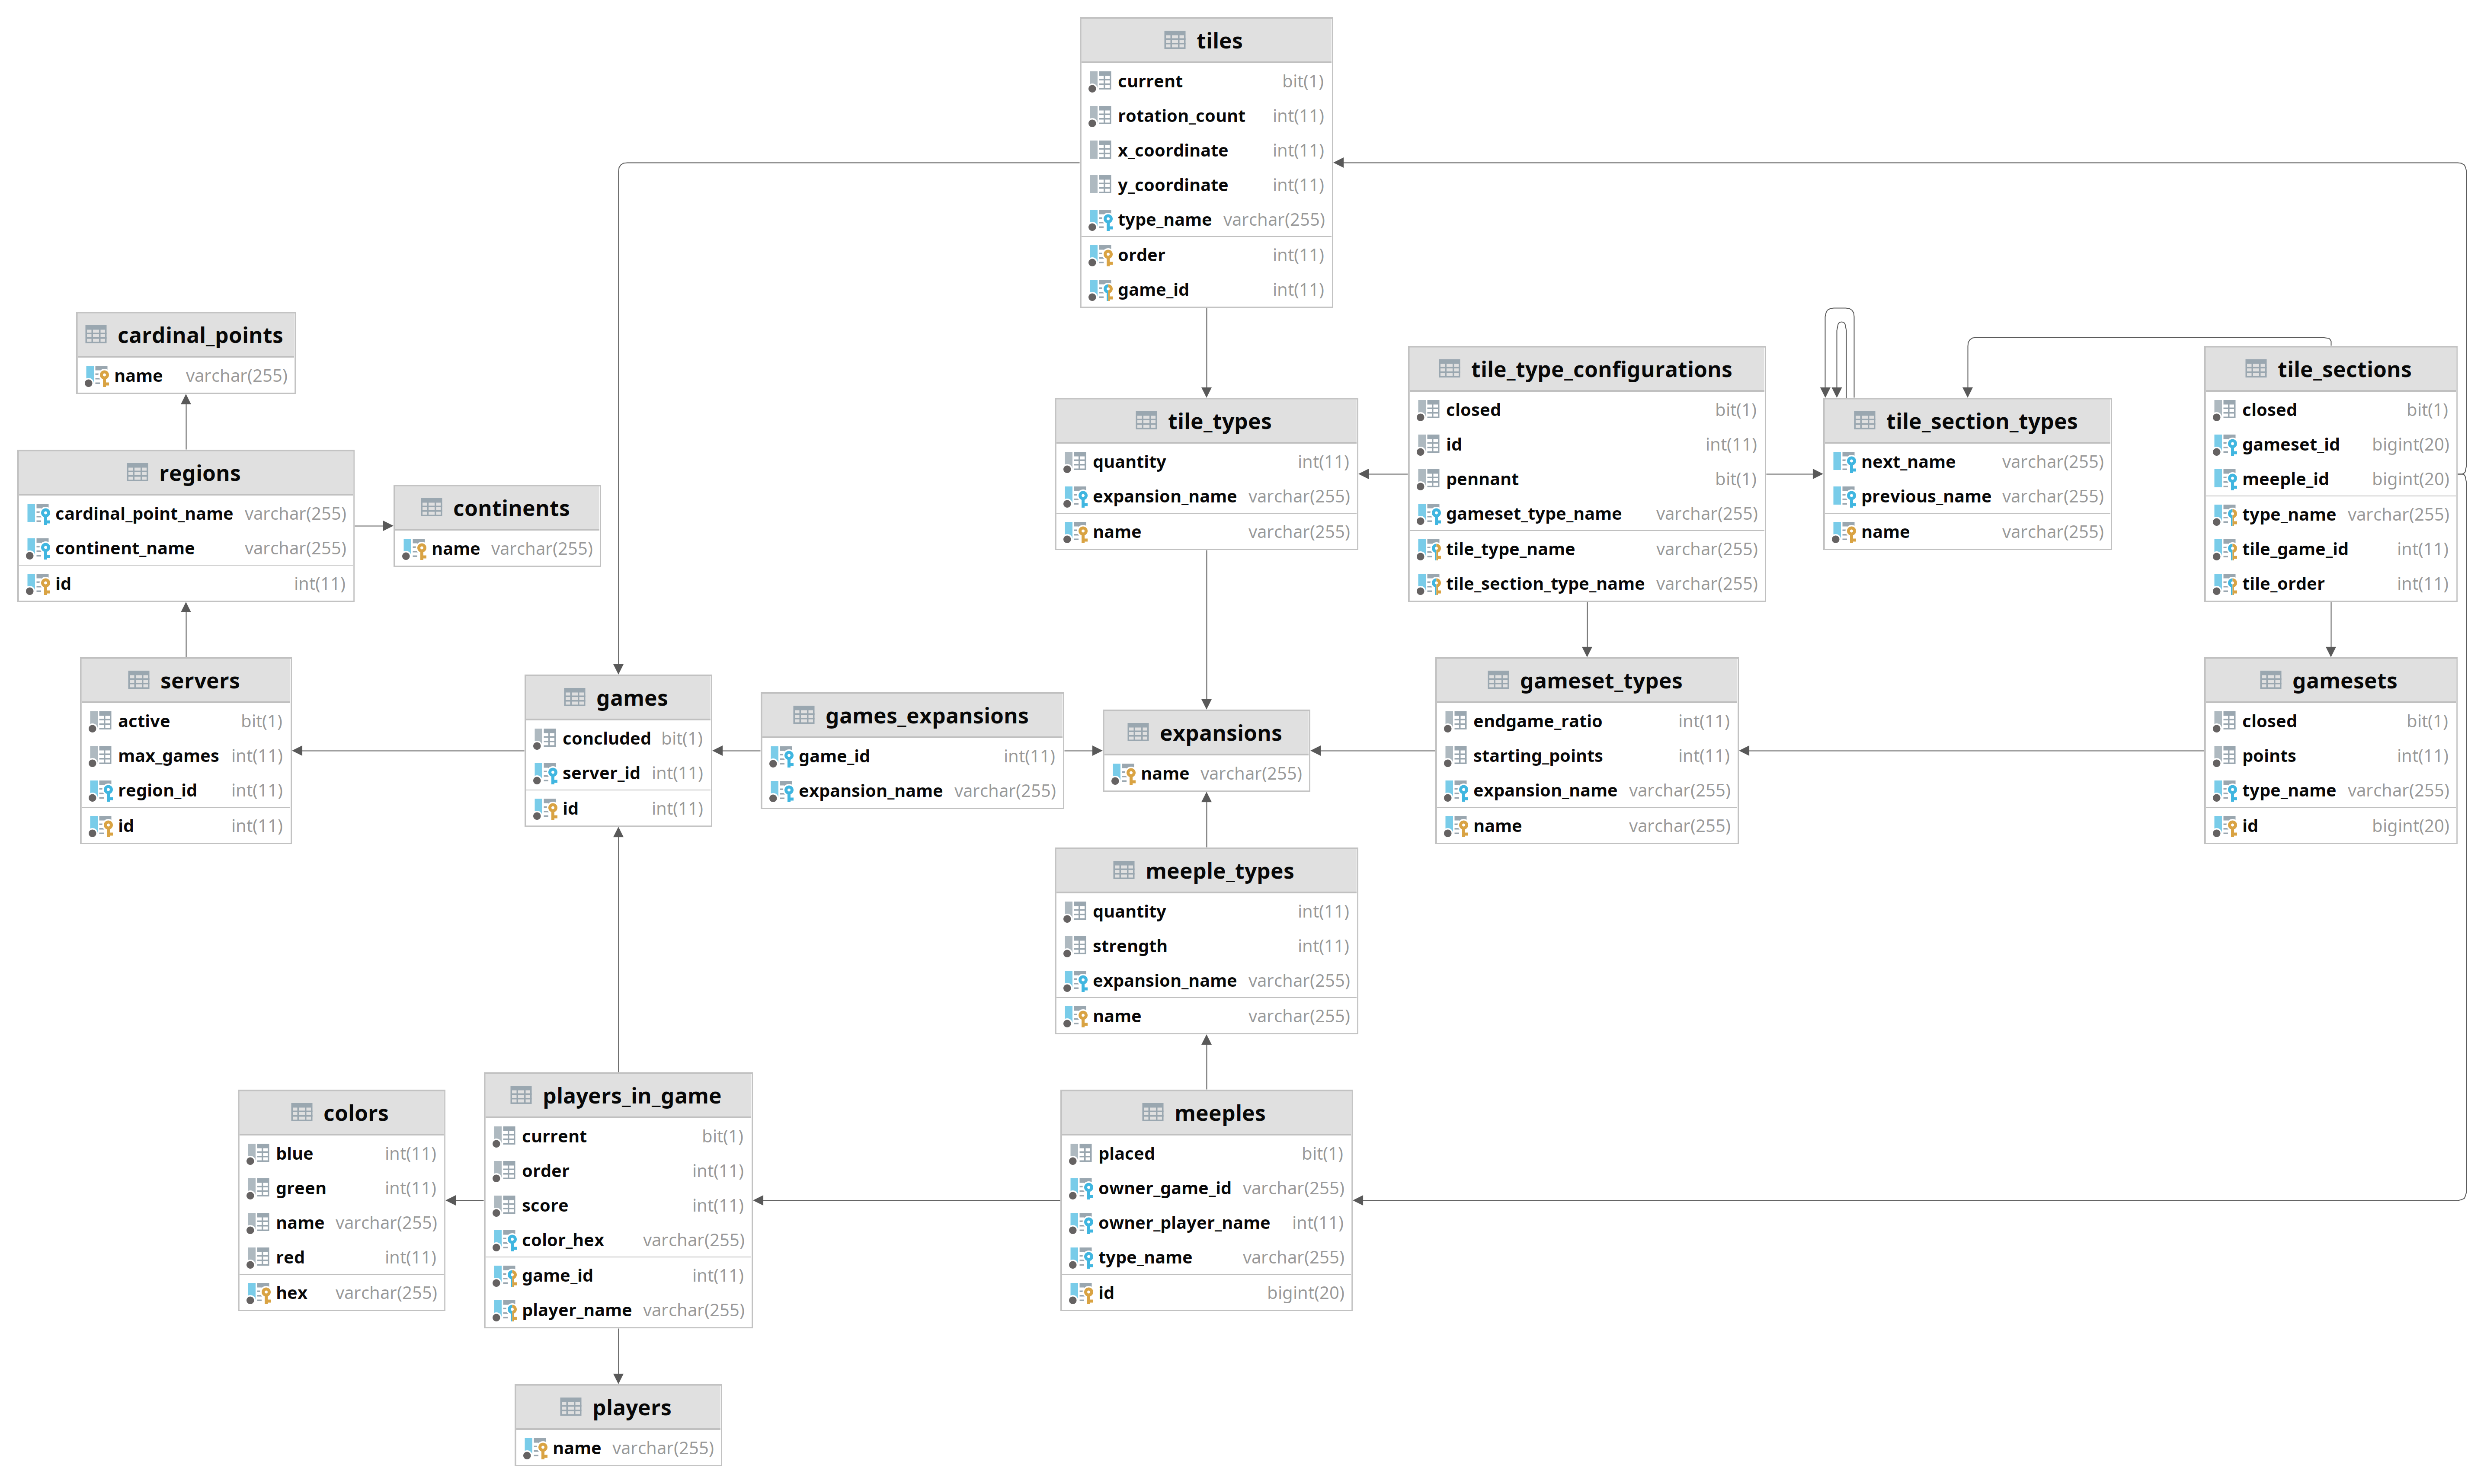
\includegraphics[scale=0.06]{images/Progettazione/relazionale.png}
    \caption{Schema concettuale finale.}
\end{figure}

\subsection{Traduzione delle operazioni in query SQL}
